\section{\vx Prototype System}
\label{sec:prototype}

%% \begin{figure}[t]
%%   \begin{center}
%%     \includegraphics[width=\columnwidth]{figures/process-model}
%%     \caption{\vx process model.}
%%     \label{fig:process_model}
%%   \end{center}
%% \end{figure}

\begin{figure*}[t]
  \begin{center}
    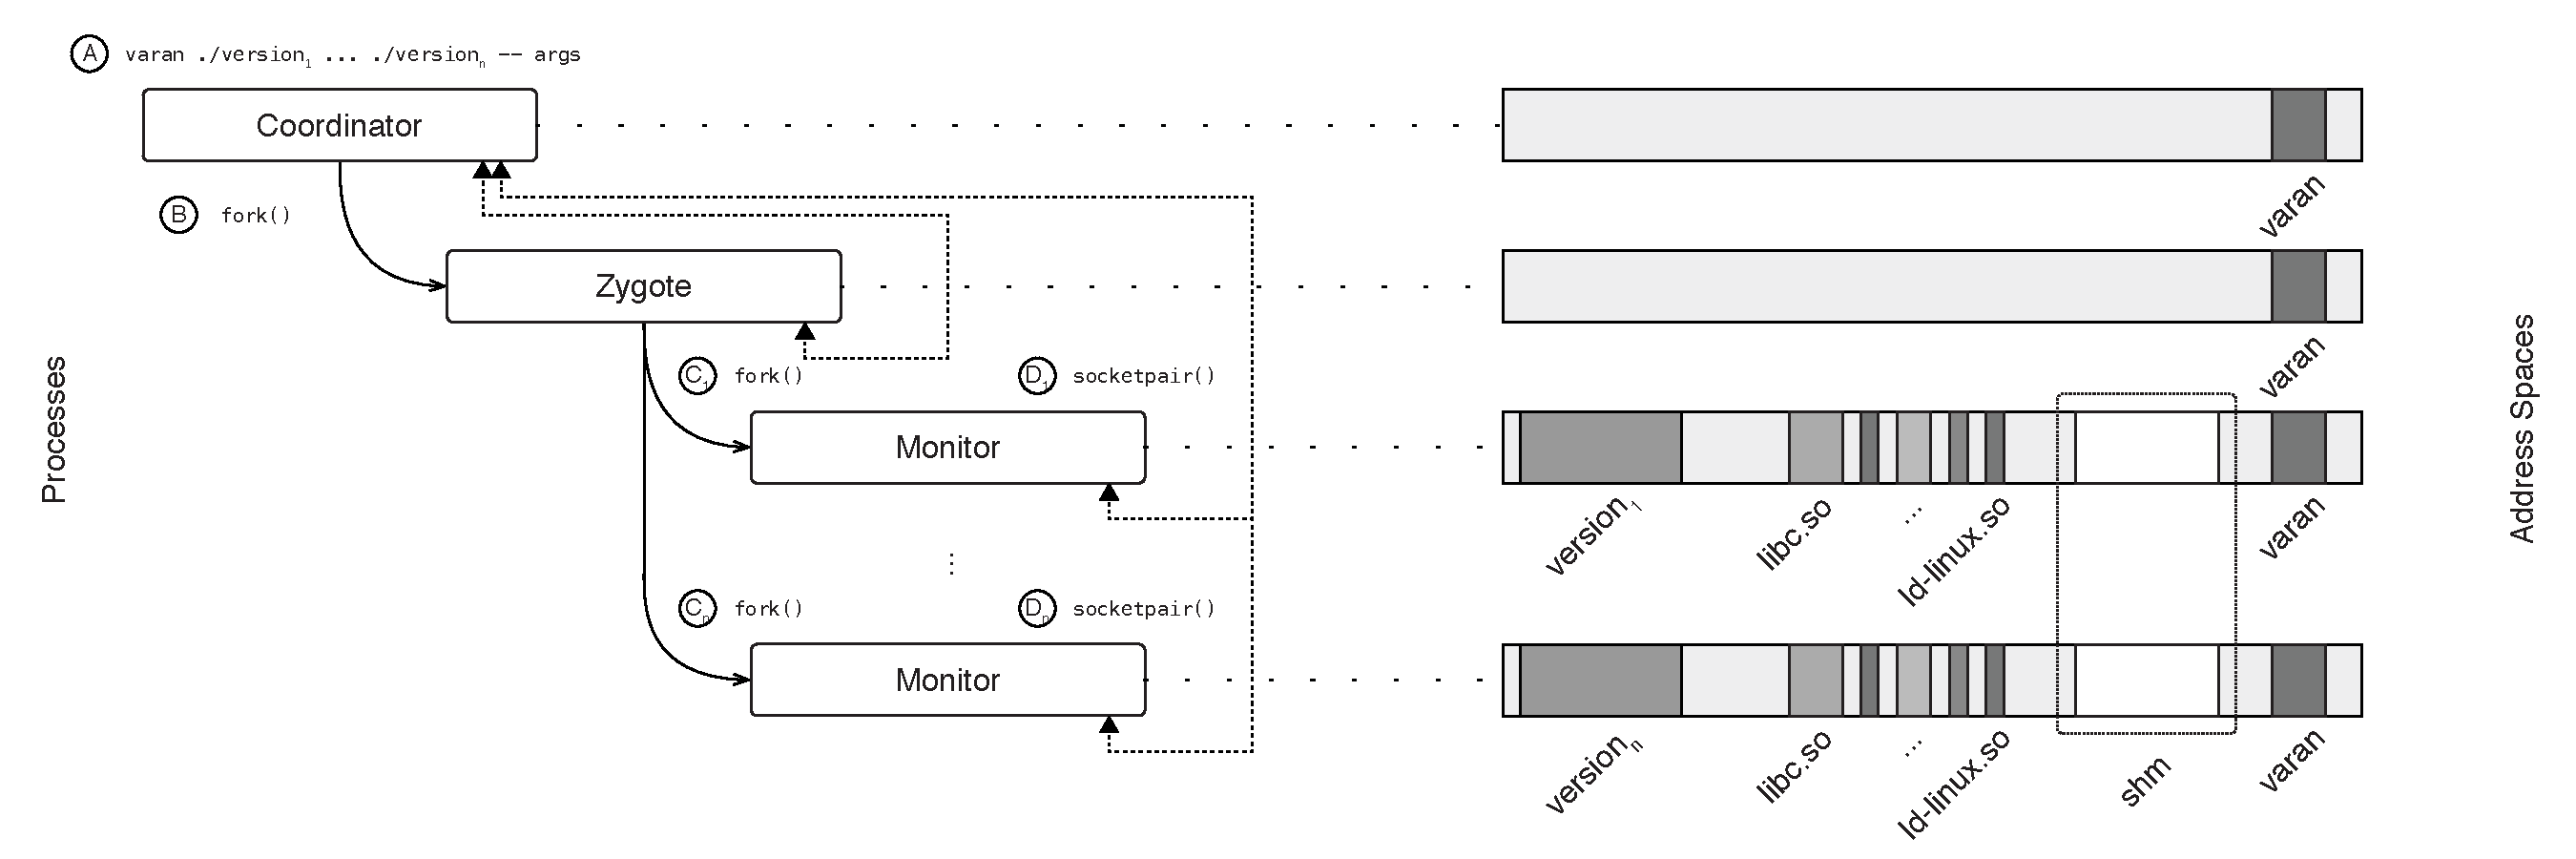
\includegraphics[width=\textwidth]{efficient-execution/figures/address-space}
    \caption{Setup of address spaces and communication channels.}
    \label{fig:setup}
  \end{center}
\end{figure*}


We have implemented our approach in a prototype, to which we will
refer as \vx, targeted at multi-core processors running x86-64 Linux.
\varan works on off-the-shelf binaries (both stripped and unstripped)
and supports single- as well as multi-threaded applications.

When it starts, \vx first sets up the address spaces of all program
versions and establishes the needed communication channels
(\S\ref{sec:setup}).  It then performs selective binary rewriting to
replace all system calls with  jump instructions
(\S\ref{sec:rewriting}).  After these initial stages, the event
streamer component of \vx ensures the coordination of the leader and
its followers (\S\ref{sec:streaming}).


\subsection{Setup of address spaces and communication channels}
\label{sec:setup}

The main steps involved in the setup of version address spaces and the
needed communication channels are shown in Figure~\ref{fig:setup}.  To
run multiple versions in parallel, the user launches \vx providing the
paths to all versions, together with any command line arguments required
to start them (Step \circl{A} in Figure~\ref{fig:setup}). \vx is built
as a statically-linked, position-independent library, to make sure it
does not stand in the way of any segments which have to be loaded by the
application at fixed addresses.

% \begin{lstlisting}[language=bash,numbers=none]
% varan -p /path/to/executable1 
%         -p /path/to/executable2 -- args
% \end{lstlisting}

%The coordinator is linked with the \vx library (\vxlib, stored in
%\stt{libvaran.so}), which will be also injected inside each version.
%\vxlib is built as a statically-linked, position-independent library,
%to make sure it does not stand in the way of any segments which have
%to be loaded by the application at fixed addresses.

The \emph{coordinator} code first creates the shared memory segment
used for communication among versions, and then spawns the
\textit{zygote} process (\circl{B}), which is responsible for starting
the individual versions. The coordinator communicates with the zygote
via a UNIX domain socket. For each version $i$ that needs to be spawned,
the coordinator sends a fork request to the zygote over this socket
pair, which includes the path to that version executable, the command
line arguments, and the end-point of a socket pair which will be used
for the subsequent communication between the coordinator and that
version (\circl{C$_i$}).
%
After receiving this request, the zygote spawns a new process, which
first finalizes the communication with the coordinator
(\circl{D$_i$}).  The coordinator then sends the shared memory
segment descriptor to this process, which maps it inside its address
space.

%% returns a process identifier to the coordinator.  The coordinator then
%% sends the rank and shared memory segment descriptor to the version.

In the final step, the new process starts executing inside the
\emph{monitor} code, which loads the specified ELF executable and sets
up the initial address space as described in the ELF headers. If the
program requires a dynamic linker, \vx loads the linker image specified
in the header as well.
%% Afterwards, \vx attaches the shared memory segment and initializes
%% the system call table based on the rank and arguments provided by
%% the coordinator.
The text segments of both the application and the dynamic linker are
then processed by the binary rewriter (\S\ref{sec:rewriting}). Finally,
\vx jumps to the application entry point as specified in the ELF header,
starting the execution of the application version.

%% \vx is operates at the thin boundary between the operating system and
%% the user-space application---\ie below the C library and the dynamic
%% linker---and lives inside the address space of the host application;
%% however, the application itself is unaware of its existence.

% The rest of this section provides some extra details regarding the
% role and implementation of the coordinator, monitor and zygote.

\boldtext{Coordinator.}  Essentially, to set up the address spaces of
the versions, the coordinator acts as a specialized preloader, inspired
by
\emph{rtldi}.\footnote{\url{http://www.bitwagon.com/rtldi/rtldi.html}}
However, the coordinator does not attempt to replace the existing
dynamic linker, which would be unnecessarily complex and may affect
compatibility with existing applications. Instead, it simply intercepts
system calls performed by the linker to enable the binary rewriter
(discussed in \S\ref{sec:rewriting}) to rewrite the code of
dynamically-linked shared libraries.  One important advantage of our
interception mechanism is that we do not make use of \ptrace to
intercept calls to the dynamic linker---instead, the binary rewriter is
used to rewrite all the system calls done by the linker with jumps into
the coordinator code.  As a result, \vx can be used in combination with
existing \stt{ptrace}-based tools such as \textit{GDB} or
\textit{strace}, which greatly simplifies debugging.

%% This also has an advantage of supporting arbitrary dynamic linkers,
%% not just the one provided by GNU C library, albeit it is going to be
%% the most common target.

%% This architecture has several advantages over other commonly
%% approaches. \vx does not require the use of dynamic linker, as
%% required by \stt{LD\_PRELOAD}. 


\boldtext{Monitor.} To ensure that \vx can be compiled as
statically-linked position-independent code, we must avoid using any
global variables (\ie those in the \stt{.data} section). One of the
consequences is that \vx cannot use any of the existing C libraries such
as \textit{GNU C Library}, as these are not typically built to support
this requirement.  Instead, \vx provides its own implementation of the
necessary C library functions based on the \textit{Bionic C
library}.\footnote{\url{https://android.googlesource.com/platform/bionic.git}}
To support the use of Linux system calls, \vx uses a modified version of
the \stt{linux\_syscall\_support.h}
header.\footnote{\url{https://code.google.com/p/linux-syscall-support/}}

%% \vxlib provides its own entry point (\ie the \stt{\_start} function),
%% which is the starting point for \vx's execution. After start, it first
%% processes the arguments passed on stack by the Linux kernel, including
%% program arguments, environment variables and most importantly the
%% auxiliary data. Then, it loads the specified ELF executable into the
%% address space. Since \vx operates as a pre-loader, it is responsible
%% for setting up the initial address space layout as described by the
%% program header. If the program being executed requires dynamic linker,
%% \vx loads the linker image specified in the program header as
%% well. The text segments of both the application and the dynamic linker
%% are then processed by the binary rewriter (\S\ref{sec:rewriting}).


\boldtext{Zygote.} While it would be technically possible for the coordinator
to create the processes in which versions run, instead of delegating this
functionality onto the zygote, this would bring some complications regarding
the communication channels: for example, the second version spawned would
inherit the communication channel between the first version and the
coordinator, which would be undesirable.  Zygote processes are already used in
popular systems such as \textit{Android} and
\textit{Chrome}~\cite{linuxzygote}---in this paper, we use the term to refer to
the concept rather than a concrete implementation, as \vx provides its own
clean-slate implementation.

After start, \vx sets up the communication subsystem (\ie the shared memory
allocator, the ring buffer) and then forks the Zygote process. The Zygote
closes all open descriptors except for the socket used as a communication
channel with the coordinator and enters the dispatch loop to wait for incoming
requests. On fork request, the Zygote receives command line arguments (\ie
\stt{argv}) and a set of file descriptors which will be available to the new
process; then forks itself and resumes to dispatch loop. The other type of
requests that Zygote supports are querying for process status (\ie equivalent
of \stt{waitpid}) and process termination (\ie \stt{SIGKILL}).

\subsection{Binary Rewriting}
\label{sec:rewriting}

To intercept system calls, \vx uses selective binary rewriting~\cite{bird}.
Unlike traditional dynamic binary rewriting implemented by tools like
DynamoRIO~\cite{dynamorio02} or Pin~\cite{pin05}, where the entire process
image is being rewritten often introducing significant performance overhead,
\vx only replaces certain instructions, in particular the instructions for
performing system calls (\ie \stt{INT 0x80} on x86 and \stt{SYSCALL} on
x86-64).  This approach has been originally implemented in
\emph{BIRD}~\cite{bird} for the Windows/x86 platform and later in
\emph{seccompsandbox}\footnote{\url{https://code.google.com/p/seccompsandbox/}}
for Linux.  Our implementation extends the
\emph{seccompsandbox}\footnote{\url{https://code.google.com/p/seccompsandbox/}}
framework for Linux.

The rewriting itself is done statically when a text segment is mapped into
memory.  (\ie \stt{mmap} system calls with executable flag, typically performed
by the dynamic linker).  \vx iterates through the text segment searching for
system call instructions using a simple x86 disassembler. Every system call
found is rewritten with a jump to an internal system call entry point. This
process is complicated by the fact that while a system call instruction is only
one byte long, a jump instruction requires five bytes. Therefore, in order to
rewrite the system call with a jump, we also need to relocate some of the
instructions surrounding the system call---\ie perform binary detouring via
trampolines~\cite{detours}.  On rare occasions when this is not possible (\eg
because the surrounding instructions are potential branch targets), we replace
the system call with an interrupt (\stt{INT 0x0}).  This interrupt is handled
by \vx through a signal handler installed during initialization, which
redirects the control flow to the system call entry point as for other system
calls.

The system call entry point first saves all registers, and then checks an
internal system call table to see whether there is a handler installed for that
particular system call; if so, it calls that handler (using a user space
calling convention), otherwise it invokes the default handler.  After
processing the system call, the entry point handler restores all registers and
returns to the original caller (using \stt{sigreturn} in the case of system
calls intercepted via an interrupt). The system call entry point also
implements support for restarting system calls, normally handled by the kernel
(\ie signaled by the \stt{-ERESTARTSYS} error code). This is used in certain
scenarios supported by \vx such as transparent failover (\S\ref{sec:failover}).

The internal system call table can be easily changed to accommodate
various application scenarios.  In particular, the only difference
between the leader and the followers is the system call table. For
example, the \stt{write} system call would be redirected in the leader
to a function that performs the call and records its result in the
shared ring buffer, while in the followers it would be redirected to a
function that reads the results from the shared buffer without making
the call.
%% \vx allows both the system call table and the default system call
%% handler to be provided by the embedder of \vx \todo{Where shall we
%%   described the possibility of \vx embedding, \ie building tools on
%%   top of \vx?}. This makes it easy to customize \vx behavior for
%% different use cases (\S\ref{sec:failover}). For our prototype, we have
%% provide three different system call tables (\ie record, replay and
%% passthrough). 
\varan  also provides a Python script which can produce new tables
and their implementations using templates.
%% ; in fact, the passthrough table was implemented using this
%% generator. We have also used the generator throughout the \vx
%% development for testing and debugging purposes.


\subsubsection{Virtual System Calls}
\label{sec:vsyscall}

The \emph{vsyscall} page and the \emph{vDSO} segment are two
mechanisms used to accelerate certain system calls in Linux. Each
process in Linux has two special segments mapped into its address
space, containing virtual system call implementations. These system
calls do not incur the context switch overhead between kernel and
user space associated with "standard" system calls.

The \emph{vsyscall} page was introduced first, but is being deprecated in favor
of the \emph{vDSO} segment.\footnote{We are referring to x86-64 version, on x86
the vDSO segment contains a function used to determine the preferred method of
making a system call} The main reason for this development is that the
\emph{vsyscall} page is mapped to a fixed address, making it susceptible to
return-oriented programming attacks~\cite{ROP:tissec12}. To address this issue,
the vDSO segment is mapped to a random address. Since the segment is
dynamically allocated, it can also support an arbitrary number of virtual
system calls (currently \stt{clock\_gettime}, \stt{getcpu}, \stt{gettimeofday}
and \stt{time}).

Virtual system calls represents one of the major limitations of
\stt{ptrace} based monitors. Since these system calls are entirely
implemented in user space, they cannot be intercepted via \ptrace.
This is an important limitation: as these system calls provide access
to timing information, they are often used as a source of
non-determinism (\eg for random number generators) and their handling
is critical for any NVX system. Despite this, previous systems either
omit discussion on virtual system call handling~\cite{mx,orchestra11}
or explicitly mention their inability to handle them~\cite{tachyon12}.

To our knowledge, \vx is the first NVX system which handles virtual
system calls, using binary rewriting. 
%In \vx, binary rewriting is also used to intercept virtual system
%calls.
Handling calls made via the \textit{vsyscall} page is easier, as
the function symbols are always mapped at the same address.  
We can therefore easily identify calls to these functions while
scanning the text segment and rewrite them to calls into our system
call table.
To handle \textit{vDSO} calls, we first need to
determine the base address of the \textit{vDSO} segment; this address
is passed by the kernel in the ELF auxiliary vector via the
\stt{AT\_SYSINFO\_EHDR}
flag.\footnote{\url{https://www.gnu.org/software/libc/manual/html_node/Auxiliary-Vector.html}}
Second, we need to examine the ELF headers of the \textit{vDSO}
segment to find all symbols.  Since these symbols are allocated at
arbitrary addresses, statically identifying calls to these symbols as
in the \textit{vsyscall} case would be complicated. Instead, we
replace the entry point of each function with a jump to dynamically
generated code which sets up the stack and then issues a call to the
\vx system call entry point as in case of regular system
calls. Furthermore, we provide a trampoline, which allows the
invocation of the original function, by moving the first few
instructions of each function to a new place, followed by a jump to
the original code. This allows \vx to take advantage of the virtual
system call mechanism to further improve performance.

%% Finally, we note that this function interception mechanism is not
%% specific to system calls and can be used to intercept arbitrary
%% functions in the target application if needed, similarly to
%% Detours~\cite{detours}.



\subsection{Event Streaming}
\label{sec:streaming}

As briefly discussed in Section~\ref{sec:overview} and graphically
illustrated in Figure~\ref{fig:architecture}, the leader records all
external events into a shared ring buffer, while the followers replay
them to mimic the leader's behavior.  External events consist
primarily of system call invocations, but also of signals.  The leader
is the only version interacting with the environment, \ie executing
the system calls, with exception of system calls which are local to
the process (\eg \stt{mmap}). % or \stt{sigaction}).

As in any NVX system operating at the level of system calls, \vx has
to be aware of the system call semantics, in order to transfer the
arguments and results of each system call.  \vx currently implements
\syscallsHandlers system call handlers which were specifically selected
to cover the common operations (file and network I/O, event
notification, process management). This has proven enough to
successfully run all applications used in our evaluation.

%, with the remaining system
%calls allowed to be executed directly by each version, which has
%proven enough to successfully run all the servers used in our
%evaluation.

%% All application instances running in parallel under \vx are assigned
%% ranks, similarly to OpenMPI~\cite{OpenMPI}. The instance\footnote{We
%%   refer to the instances rather than a process as application may have
%%   multiple threads/subprocesses} with rank 0 is denoted as
%% \emph{leader} while all other instances are denoted as
%% \emph{followers}. 


%% When followers would execute a system call under normal execution, now
%% they simply return a value from the event stream (\ie the return value
%% of the system call executed by the leader).

% \vx recognizes several different types of events:
% \begin{inparaenum}[(i)]
% \item \emph{syscall} for the system call entry,
% \item \emph{sysret} for the system call exit,
% \item \emph{signal} for an interceptable signal,
% \item \emph{exit} for the process exit.
% \end{inparaenum}
% Furthermore, it is possible to add other types of events if necessary.

%% Each event has a fixed size of 64 bytes where first byte is
%% used as an event type.  The size has been deliberately chosen to be
%% fit into a single cache line on modern x86 CPU (see \S\ref{sec:ipc}
%% for more details).

\subsection{Inter-process Communication}
\label{sec:ipc}

%% \begin{structure}
%% \item Sending events from one process to other without the use of system
%% calls to avoid the additional overhead
%% \item Shared memory queues for process to process communication
%% \item Custom shared memory allocator with reference counting
%% \end{structure}

Since one of our primary goals for \vx was to minimize the performance
overhead, to avoid additional system calls being made during system call
handling (\S\ref{sec:overview}), we have designed an interprocess communication
mechanism which does not use system calls (\eg socket-based communication
primitives).

\subsubsection{Shared ring buffer}
\label{sec:ring}

For fast communication, the leader and its followers share a common
ring buffer of fixed size, which is held entirely in memory.  Our
initial solution used a separate shared queue for each
process~\cite{fastforward,mcringbuffer}, with the
%% Shared memory queues are often used for fast core-to-core
%% communication in high-performance applications.
coordinator acting as an event pump---reading events from the leader's
queue and dispatching them into followers' queues.  This approach
worked well for a low system call rate, but at higher rates the event
pump quickly became a bottleneck.  
% Furthermore, although we used a
% state-of-the-art shared queue implementation~\cite{bqueue}, we still
% experienced a large performance overhead for system call
% interception---over $20\times$ for a worst-case microbenchmark,
% compared to $4\times$ in the final implementation.

As a result, we have instead opted for a design based on Disruptor
pattern~\cite{disruptor} which uses a shared ring buffer allowing concurrent
access by multiple producers and consumers, eliminating the need to dispatch
events among queues, and thus improving both performance and memory
consumption.  Our implementation uses C11 atomics, 
in combination with cache aligning to
achieve maximum performance with minimal use of locking (locks are used only
during memory allocation and deallocation).

The ring buffer is used to stream events between processes. Each event
has a fixed size of 64 bytes; the size has been deliberately chosen to
fit into a single cache line on modern x86 CPUs.  This is sufficient
for sending signals and system calls for which all arguments are
passed by value (on x86-64, a system call can have up to six arguments
of eight bytes, to fit into general purpose registers).  However, for
system call arguments passed by reference, the payload might have
variable size and can be potentially larger than the event itself.  In
this case, we use events to only transfer shared pointers, which
identify memory shared across versions.


\subsubsection{Transferring file descriptors and leader replacement}
\label{sec:leader-repl}

Apart from the ring buffer, each version has a \textit{data channel},
implemented using UNIX domain sockets.
% Together, the ring buffer and data channel form an \emph{event
% stream} which is a primary communication mechanism for exchanging
% events among instances.
The data channel is used to send information which cannot be
transferred via shared memory, in particular open file descriptors.
Whenever the leader obtains new file descriptor (\eg by opening a
file), it sends this descriptor to all followers, effectively
duplicating the descriptor into their processes. This is a crucial
mechanism which enables the leader to be replaced transparently when
it crashes. When the leader crashes, the follower that is elected as
the new leader can simply continue executing using existing
descriptors (\eg responding to requests coming over network) without
any disruption in service.

% Currently, UNIX domain sockets do not support broadcast, so the leader
% communicates with the followers via the coordinator, which then sends
% the descriptor separately to all followers.  However, there are
% proposals to add broadcast support for UNIX domain
% sockets,\footnote{\url{https://lkml.org/lkml/2012/2/20/208}} which would
% simplify the design of our prototype and further improve performance.


\subsubsection{Multi-process and multi-threaded applications}
\label{sec:threading}

Handling threads is crucial in supporting many modern applications. To
alleviate non-determinism issues due to scheduling, \vx enforces
system call ordering across all threads in all variants by using a
single shared ring buffer.  Each event sent through the ring buffer is
annotated with an internal thread ID. When reading events from the buffer, each
thread checks the ID of every new event and blocks if the event ID does not
match its own.  Since our ring buffer implementation (\S\ref{sec:ring}) allows
concurrent writes by multiple producers without the need for expensive
synchronization, the use of a single shared buffer does not hinder the
application performance. 

When a new thread is spawn, a new socket pair is established between the thread
and the coordinator. The leader then continues execution, but the coordinator
waits until all followers spawn a new thread, establishing appropriate socket
pairs for communication, and setting up the thread to read events from the
shared ring buffer.

Our mechanism resembles existing deterministic multi-threading (DMT)
mechanisms~\cite{coredet:asplos10,dthreads:sosp11}. The guarantees
provided by \vx are weaker than those typically provided by these
systems as we do not enforce ordering across atomics-based
synchronization primitives.

The use of a single shared buffer presents a problem when one or more threads
perform a system call which blocks for a long period of time. In such case, the
other threads could run out of space in the ring buffer. Since the ring buffer
uses busy waiting, the following threads would also waste resources. To overcome
this problem, we have introduced a concept of \emph{waitlock}. Whenever the
following thread makes a blocking system calls, it acquires the waitlock. Such
thread is no longer holding a position in the ring buffer and it blocks until it
receives a notification from the leading thread when the waiting thread wakes up
and continues execution. The waitlocks are internally implemented using a
combination of C11 atomics and futexes~\cite{futex} for efficiency.

% However, this weaker form of determinism
% does not typically pose a problem for real-world applications as long
% as they are properly synchronized.  Note that data races resulting
% from missing or incorrect synchronization can cause followers to issue
% a different sequence of system calls from the leader.  If this
% happens, we could either try to apply one of the rewriting rules
% (\S\ref{sec:patternmatching}), or terminate the follower.
%
However, we have not detected any system call divergences caused by
related data races in our benchmarks, which include multi-threaded
applications (\eg \redis), similar to the experience reported for
prior NVX systems.  However, shall this become a problem, we could
address it by employing a stronger form of determinism similar to
existing DMT systems.

%% Each instance also has a dedicated \emph{service channel}, similarly
%% to the data channel implemented using UNIX domain sockets. The service
%% channel is used to transfer commands and service requests between
%% coordinator and the instance.

%% One such example are \stt{fork} and \stt{clone} system calls. The new
%% process spawned as a result of these system calls needs to have its
%% own data and service channel. The parent process is responsible for
%% creating these using a \stt{sockepair} system call. One end of each
%% pair is inherited by the new process while the other end is sent to
%% the coordinator where it is associated with the new process.

%Note that data races resulting from missing or incorrect
%synchronization can cause followers to issue a different sequence of
%system calls from the leader.  If this happens, that follower would
%have to be terminated.  We first note that \vx has not detected any
%system call divergences caused by data races in our benchmarks (which
%include many popular applications such as \apache, \nginx, and \redis),
%so this might not be such an important aspect in practice.  Prior NVX
%systems do not address this problem either, likely due to a comparable
%experience.

%However, we envision two possible solutions.  The first one would be
%to use deterministic multi-threading (\eg
%Dthreads~\cite{dthreads:sosp11}).  The second solution would be to
%allow developers to document any benign races as rewrite rules
%(cf. \S\ref{sec:patternmatching}).

\subsubsection{Memory allocation scheme}  

Efficient shared memory allocation plays an important role in a system
like \vx.  We use a custom shared memory pool allocator
implementation, similar to the one used by
OpenMPI.\footnote{\url{http://www.open-mpi.org/}} The shared memory
allocator uses the notion of buckets for different allocation sizes,
where each bucket holds a list of segments, and each segment is
divided into chunks of the same size; each bucket holds a free list of
chunks.  When there are no more unused chunks in a bucket, the
allocator requests a new segment from the memory pool, and divides it
into chunks which are then added to the free list. Each bucket also
has a lock associated with it which has to be held prior to an
allocation from that bucket. 
% While this design is relatively simple,
% it performed well in our benchmarks. We also experimented with
% more advanced designs (\eg using different allocation strategies for
% smaller and larger blocks), but the basic allocator always
% outperformed all other implementations.  

%% However, we believe it might still be possible to come with a more
%% specialized allocation strategy which would further improve the
%% performance of \vx, and this is something we would like to address in
%% our future work.

%% The critical part of many systems which use shared memory for
%% communication is deallocation. There are various solutions to this
%% problem. One possibility is to use some form of garbage collection,
%% such as reference counting. Unfortunately, this solution is not
%% applicable in our case since the leader is not aware of any of the
%% consumers processing its events making it difficult to consistently
%% manage the reference counts. The original Disruptor implementation,
%% which targets the Java runtime simply relied on the garbage collector
%% provided by the virtual machine. Unfortunately, this solution is not
%% applicable in our case either. Instead, we have extended the C-based
%% Disruptor implementation to notify a follower if it is the last one
%% that processes an event. \todo{how?}  If that is the case, the
%% follower is responsible for freeing the associated memory. This
%% solution does not add any overhead and does not require any
%% modifications to the allocator.

% This property allows us sharing memory between individual application
% instances without explicitly tracking which instance is responsible for
% deallocation, or using the back channel to notify instance that the block is
% available for deallocation as in the case of OpenMPI

\subsection{Rewrite rules for system call sequences}
%\subsubsection{System call filtering and rewriting}
\label{sec:patternmatching}

\vx uses BPF filters to implement the system call rewrite rules introduced in
Section~\ref{sec:rw}.  BPF is a machine language for writing rules and an
interpreter shipped with many UNIX implementations, including Linux and BSD.
BPF filters have been traditionally used to filter network packets, but
recently also for system call filtering as a part of seccomp "mode 2" (also
known as seccomp-bpf).

We have integrated a BPF interpreter in \vx to allow for system call rewrite
rules. Our implementation is based on the Linux kernel code which has been been
ported to user space and extended for NVX execution.  This required adding a
new return value \lstinline`SECCOMP_RET_REPLACE` where the bottom 16-bits of
the return value specify the new system call number the original system call is
going to be rewritten to.  Since these extensions does not add any new
instructions or extend the semantics of the BPF language, the
\lstinline`bpf_asm` tool can be used to compile the filters into a binary form.
This can be then loaded into \vx on start through a command line option.

The use of BPF has a number of advantages.  First, it does not require
the user to modify and recompile the monitor on every rule
change. This is particularly important as rewrite rules are likely
going to be application specific. Second, the BPF machine language was
designed to be simple enough to prevent a large class of errors---\eg
all filters are statically verified on load to ensure termination.
(\ie every filter has to end with a \lstinline`ret` instruction).

We also argue that the choice of BPF as a language for stream rewriting rules
makes it easier to adopt by administrators, the most likely users of \vx,
compared to some other more esoteric languages such as Haskell~\cite{tachyon12}.

\begin{lstlisting}{language=[bpf]Assembler,caption={Example of a BPF rewriting rule}}
ld [0]                /* offsetof(struct seccomp_data, nr) */
jne #1, good          /* __NR_write */
bad: ret #0           /* SECCOMP_RET_KILL */
ldi #18               /* __NR_pwrite */
add #0x00070000       /* 18 + 0x00070000 */
ret %a                /* SECCOMP_RET_REWRITE */
good: ret #0x7fff0000 /* SECCOMP_RET_ALLOW */
\end{lstlisting}
